\section{Related Work}
\label{sec:relWork}

This chapter presents the relevant background knowledge and show approaches from other scientific paper.

\subsection{ISO/IEC 27004:2009}

This present thesis based the requirements of Risk measurement of ISO 27004, among other things. ISO 27004 is a international security standard from the ISO 27000 \cite{DBLP:conf/euspn/MeriahR19} family which guides on continious basis evaluation methods. The present ISO can be related with ISO 27001 or used as a standalone standard. In ISO 27001 it is declared as a requirement where the effectiveness must be measured of a Information Security Management System \cite{barabanov2011information}. The ISO 27004 standard specifies what to be measured, when the measurement is needed and types of measurement \cite{lundholm2011design}. Barabanov et. al \cite{barabanov2011information} and Tarnes \cite{tarnes2012information} describe in their works the different properties of ISO/IEC 27004:2009 for Risk measurement. Tarnes shows the information security measurement model which is shown in Figure \ref{fig:is_measurement_model}.

\begin{figure}[h!]
  \centering
  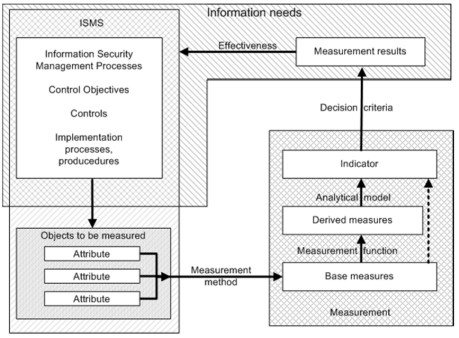
\includegraphics[width=8cm]{pictures/is_measurement_model.jpg}
  \caption{The information security measurement model \cite{tarnes2012information}}
  \label{fig:is_measurement_model}
\end{figure}

For this thesis the objects to be measured and the measurement are the important parts of the information security measurement model. The measurement method is the SMF which measure based on different properties that are derived from risk indicators \ref{sec:risk_indicators}. The attributes in Figure \ref{fig:is_measurement_model} are the properties in the SMF.

\subsection{Security risks in context of Machine Learning}

Xiao et. al \cite{DBLP:conf/sp/XiaoLZX18} evaluate the security risks in deep learning for common frameworks i.e. TensorFlow. Xiao et. al uses the framework sample applications along the frameworks. One
statement of Xiao et. al is that the named frameworks TensorFlow, Caffe and Torch are implemented with many lines of code which make them vulnerable for many security vulnerabilities i.e. heap overflow
or integer overflow. Xiao et. al work is only in context of deep learning e.g. only for neural networks.

\subsection{Risk assessment in context of Machine Learning}

Paul Schwerdtner et. al \cite{DBLP:journals/corr/abs-2011-04328} present in their
work a framework to evaluate ML model by input corrupted data. This thesis discuss
this paper as an approach to estimate where the SMF could be used for.

\subsection{Adversarial-Robustness-Toolbox}

For this thesis the technical framework Adversarial-Robustness-Toolbox (ART)
\cite{art2018} is a main component.

\subsection{Approaches from Jakub Breier et. al and Paul Schwerdtner et. al}

This present thesis is divided into two approaches.
Jakub Breier et. al \cite{DBLP:journals/corr/abs-2012-04884} propose in their paper
different proposals to measure risks with different aspects. \\
Paul Schwerdtner et. al \cite{DBLP:journals/corr/abs-2011-04328} is the second approach of this thesis.
